\section{Experiments and Analysis}
\label{sec:experiments}
This section empirically validates the core hypothesis of \textsc{XDomainBench}: as knowledge compositions increase in order and structural complexity, LLM performance degrades in interactive interdisciplinary scientific reasoning, and the degradation can be diagnosed through trajectory patterns and the failure phenomena they precipitate.

\subsection{Evaluation setup}
\label{sec:exp_setup}

\textbf{Evaluation suite and interactive protocol.}
We evaluate models on a sampled evaluation suite of \textsc{XDomainBench} episodes, constructed with stratified sampling to ensure coverage across domains, compositions, and trajectory patterns.
All experiments use a standardized interactive protocol with a history mechanism: each turn's context includes previous turns, allowing later turns to be influenced by earlier ones.
We evaluate diverse LLMs spanning frontier proprietary systems and open-weight models, all queried in a zero-shot setting.
Detailed sampling quotas, coverage statistics, and protocol details are in Appendices~\ref{app:dataset_stats}, \ref{app:sample_composition}, and \ref{app:controller}.

\textbf{Metrics.}
%Following holistic and robustness-oriented evaluation principles~\citep{liang2022helm,chang-etal-2023-survey,ribeiro-etal-2020-beyond,kiela-etal-2021-dynabench,schlangen-2021-targeting}, we report a minimal yet diagnostic set of metrics.
For \textbf{turn-level} correctness, we use \textbf{Recall (R)} and \textbf{F1-score (F1)}.
For \textbf{session-level} success, we use \textbf{SessionSuccess@$\tau$}, which marks an episode successful if its turn-correctness rate exceeds a fixed threshold $\tau$.
Detailed metric definitions, scoring procedures, and implementation details are provided in Appendix~\ref{app:scoring}.

\subsection{Main results: degradation with composition}
\label{sec:main_results}

Table~\ref{tab:overall_scaling} and Figure~\ref{fig:radar_scaling} summarize overall performance as composition order increases from $k=1$ to $k=4$.

\paragraph{Composition order effects.}
Across all models, higher-order compositions consistently degrade performance: turn-level accuracy (Recall and F1) and session success rate (SessionSuccess@$\tau$) decline as $k$ increases from 1 to 4.
The degradation accelerates non-linearly at higher $k$ values, indicating that cross-domain integrative reasoning becomes increasingly challenging as the composition space dimension grows.
Meanwhile, the cognitive load of combining multiple domains compounds rather than accumulates linearly, like large models show moderate drops from $k=1$ to $k=2$ but steeper declines at $k=3$ and $k=4$.
Complete breakdowns by exact domain sets, task types, and trajectory patterns are provided in Appendix~\ref{app:full_results}.

\textbf{Model-type differences.}
Large models maintain relatively stable performance with moderate variance across $k$, while small models exhibit steeper degradation, with variance increasing as $k$ grows.
Meanwhile, MoE models demonstrate exceptional performance, consistently outperforming both large and small models across all $k$ values and metrics, with particularly strong performance in SessionSuccess@$\tau$.
This pattern indicates that smaller models struggle more with the cognitive load of higher-dimensional domain compositions, while MoE architectures excel at handling complex compositional reasoning tasks.

\begin{table}[t]
\centering
\caption{Semantic-evaluation robustness under increasing composition order,
showing judge-based evaluation preserves the same degradation trend as token-level Recall.}
\label{tab:judge_robustness}
\vspace{-1mm}
\resizebox{0.98\linewidth}{!}{
\begin{tabular}{lccccc}
\toprule
Metric & $k=1$ & $k=2$ & $k=3$ & $k=4$ & Drop Var. \\
\midrule
Token Recall & 31.3 & 28.0 & 24.1 & 21.9 & 0.021 \\
Judge Acc. & 37.1 & 33.0 & 29.0 & 26.8 & 0.018 \\
\bottomrule
\end{tabular}
}
\end{table}

To verify that the observed collapse is not an artifact of lexical overlap, 
we evaluate model outputs using a judge-based semantic correctness score.
As shown in Table~\ref{tab:judge_robustness}, the semantic judge yields higher absolute scores, 
as expected under a more relaxed criterion, but preserves the same monotonic degradation as the composition order increases.
This suggests that token-level Recall provides a stricter measurement of the same underlying failure pattern, 
rather than manufacturing the collapse through surface-form brittleness.

\begin{figure}[!t]
  \centering
  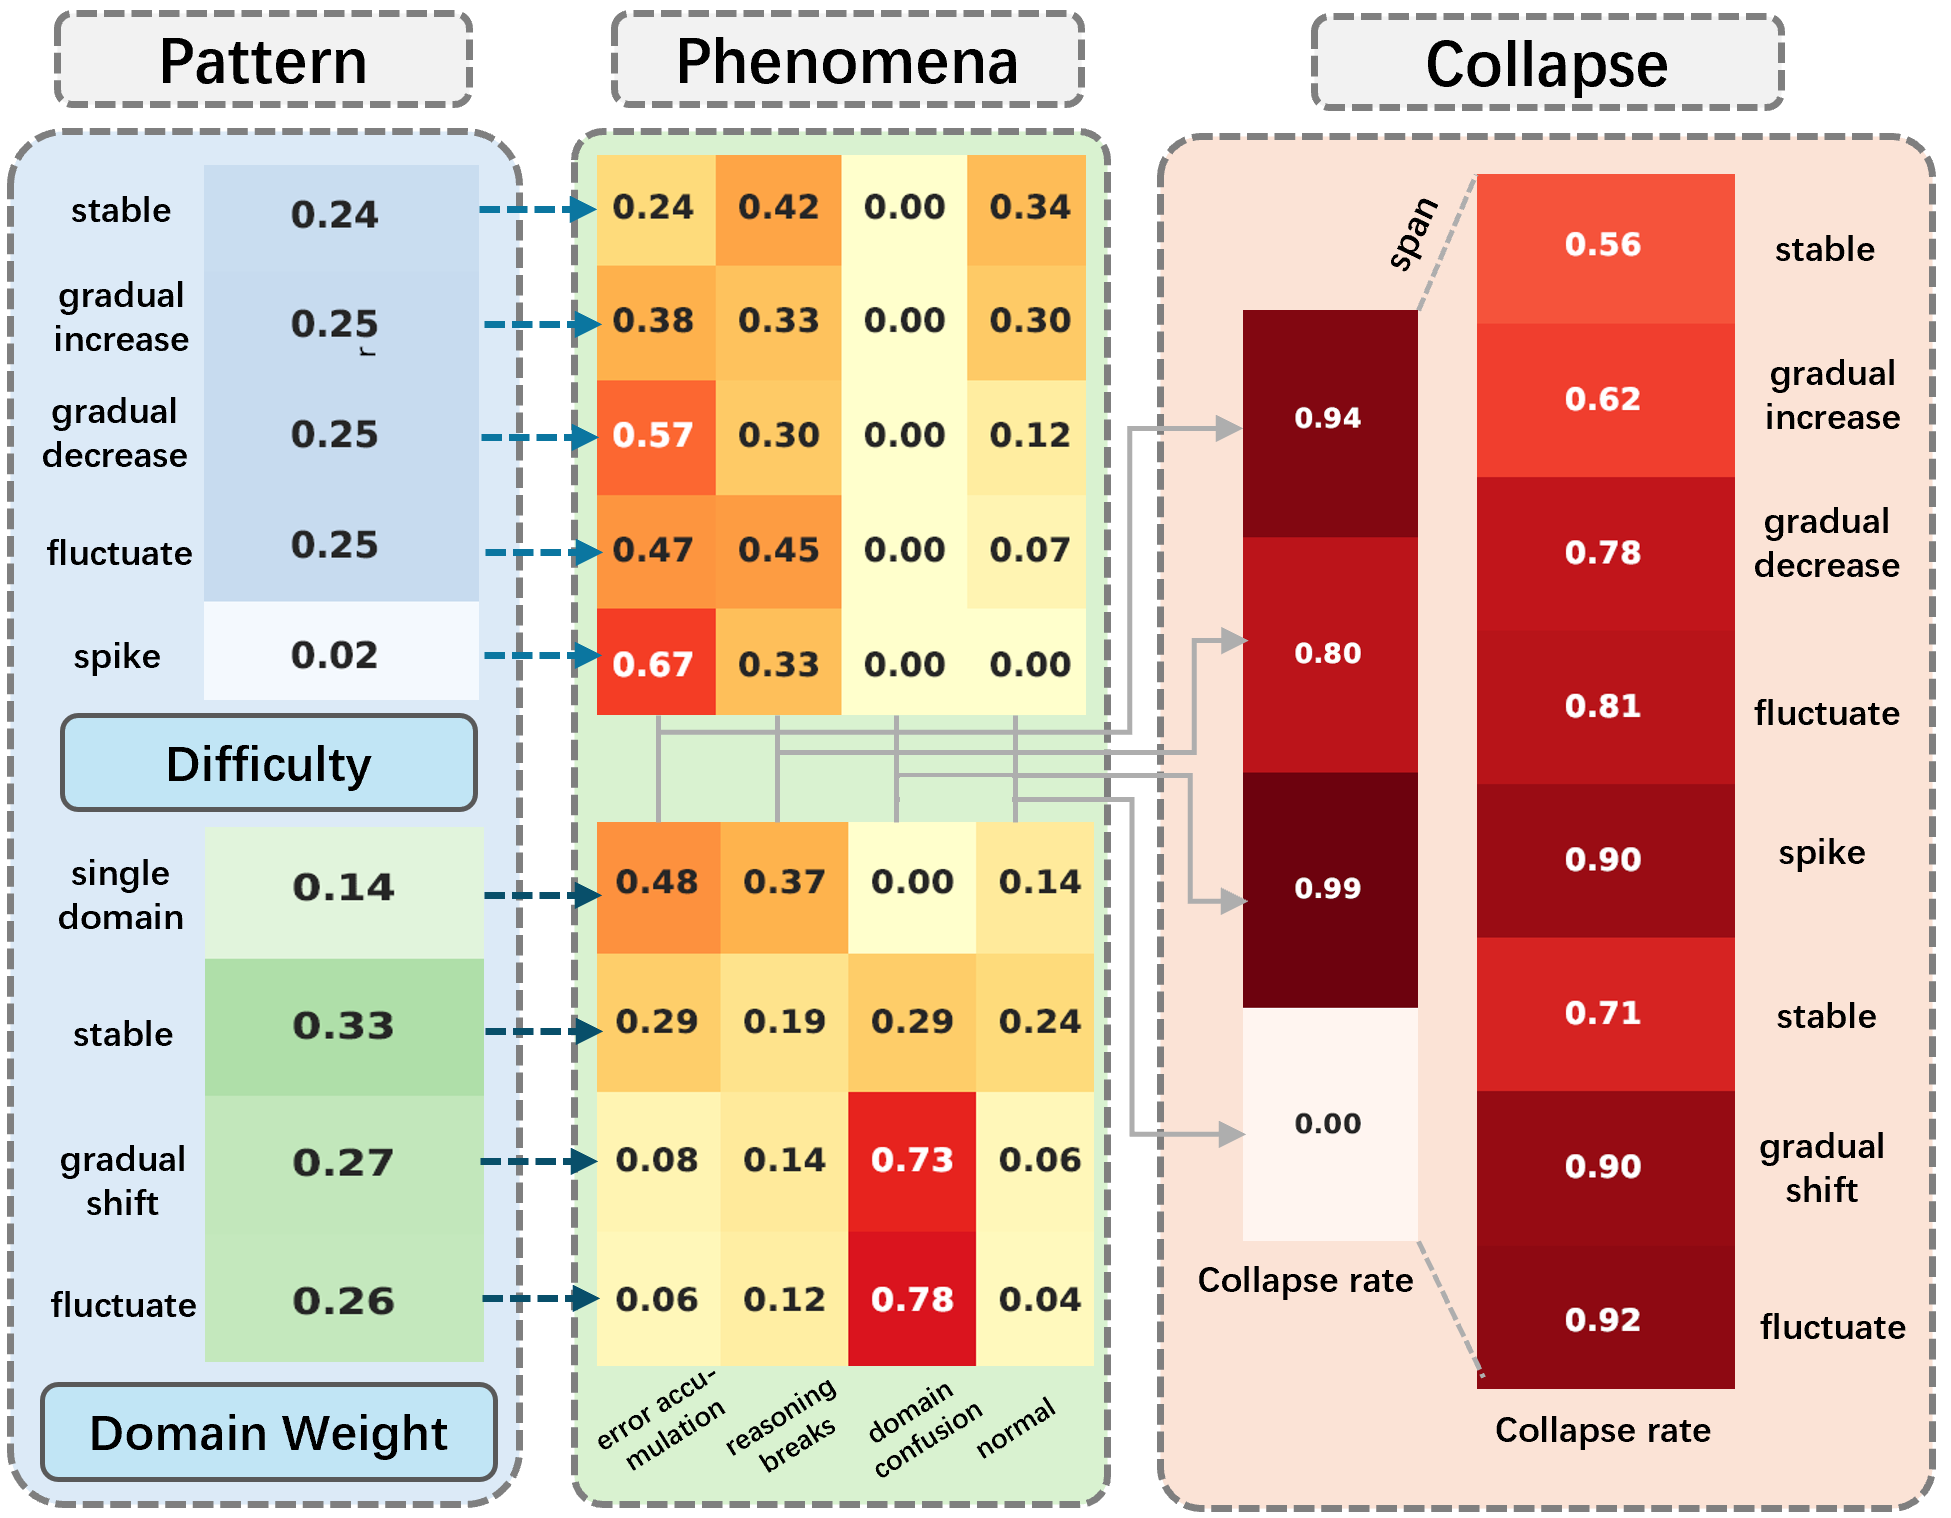
\includegraphics[width=1.00\linewidth]{figures/mechanism_summary_left.png}
  \vspace{-3mm}
  \caption{\textbf{Mechanism summary: pattern distribution, pattern $\rightarrow$ phenomena, and pattern/phenomena $\rightarrow$ collapse associations.}
  All statistics are averaged across all models.}
  \vspace{-1mm}
  \label{fig:mechanism_summary_left}
\end{figure}

\subsection{Diagnostic analysis}
\label{sec:diagnostic}

The aggregate degradation combines two sources: (i) \textbf{direct difficulty increase} induced by domain composition, and (ii) \textbf{indirect interaction-amplified} failures arising from particular difficulty and mixture trajectory patterns.

\subsubsection{Direct mechanism}
\label{sec:paired_drop}

The direct mechanism reflects \textit{insufficient capability for handling compositional problems} as domain combinations increase.
Following the construction method in Section~\ref{sec:episode_construction}, the first turn of each composed episode is instantiated from the same single-domain seed pools as corresponding $k{=}1$ episodes, enabling direct comparison.
For a $k$-domain composition ($k\in\{2,3,4\}$), we compare turn-1 correctness on composed episodes against $k$ single-domain baselines, defining the \emph{composition drop} as the difference between composed turn-1 performance and the mean of constituent baselines.
Figure~\ref{fig:turn1_barplot} visualizes turn-1 performance and difficulty across composition orders and task types.

Across all models, composing domains induces immediate performance decline, with magnitude increasing as $k$ grows, indicating that combining disciplines imposes an integrative load \emph{prior to} any multi-turn error propagation.
The decline is consistent across task types, with difficulty increasing systematically.
Detailed turn-1 before/after comparisons for all domain sets are reported in Appendix~\ref{app:combo_breakdown}.

\begin{figure}[!t]
  \centering
  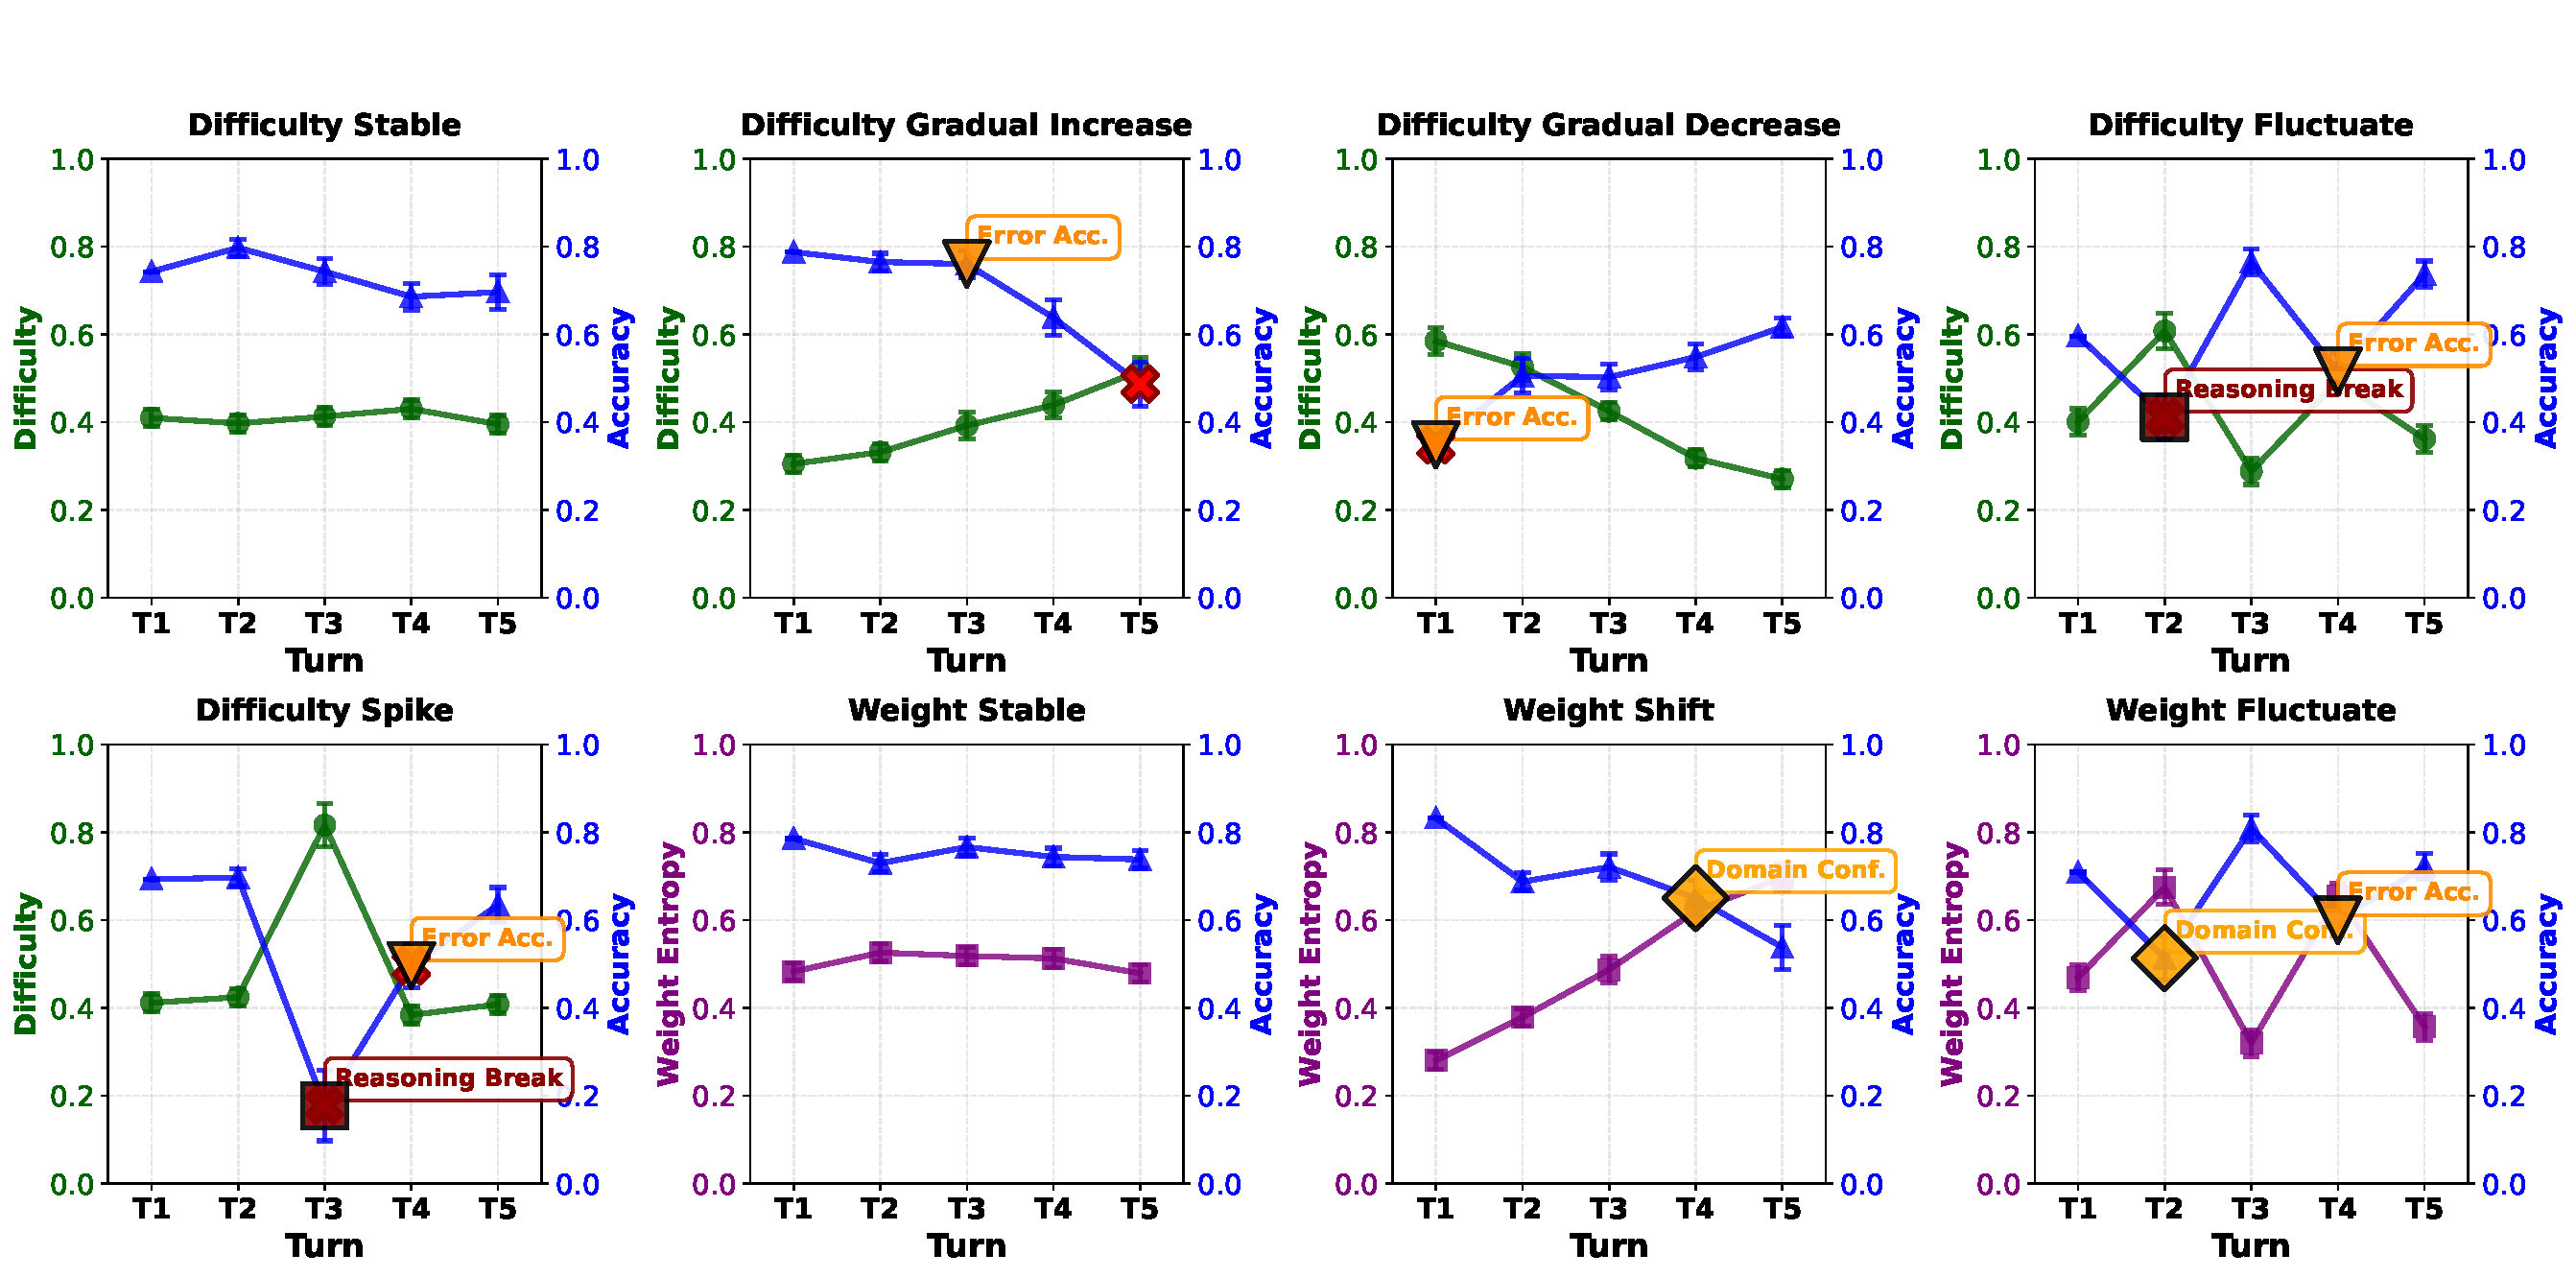
\includegraphics[width=\linewidth]{figures/mechanism_summary_right.pdf}
  \caption{\textbf{Trajectories of pattern and performance for eight pattern types.}
  Each panel shows difficulty or weight entropy and accuracy evolution across turns, illustrating how pattern characteristics trigger specific failure phenomena.
  }
  \vspace{-1mm}
  \label{fig:mechanism_summary_right}
\end{figure}

\subsubsection{Indirect mechanism}                                                                                                                                                                                                               
\label{sec:mechanism}

The indirect mechanism reflects \textit{performance degradation induced by domain-mixture dynamics in multi-turn interactive scenarios}.
We analyze how interactive trajectory patterns in difficulty $\{\delta_t\}$ and domain-mixture $\{w_t\}$ signals indirectly induce failure phenomena, ultimately leading to session-level collapse.
We group episodes into representative pattern types using drift and volatility statistics, and examine the chain from trajectory patterns to failure phenomena to session collapse.

Quantificationally, Figure~\ref{fig:mechanism_summary_left} embodies the mechanism across all models: pattern distributions, pattern-to-phenomena associations, phenomena-to-collapse links, and pattern-to-collapse probabilities.
The middle columns map patterns to failure phenomena, showing that different patterns trigger different phenomena at varying rates (e.g., gradual decrease patterns strongly associate with error accumulation, while fluctuate patterns trigger both error accumulation and reasoning breaks).
The rightmost columns show that all three failure phenomena lead to high collapse rates, and that pattern-to-collapse probabilities follow the expected trend: stable patterns have lower collapse rates while more volatile patterns (fluctuate, spike) have higher rates.

Qualitatively, Figure~\ref{fig:mechanism_summary_right} illustrates trajectories for each pattern type, showing how difficulty or weight entropy evolves across turns alongside accuracy.
These trajectories demonstrate how specific pattern characteristics lead to different failure phenomena: gradual decrease patterns show early high difficulty causing error accumulation, spike patterns show sudden difficulty spikes triggering reasoning breaks that contaminate subsequent turns, and fluctuate patterns exhibit multiple phenomena due to volatility.

\paragraph{Diagnostic interpretation.}
Our analysis should be interpreted as controlled diagnostic attribution rather than a full causal intervention study.
The paired turn-1 comparison isolates a direct composition overhead before multi-turn propagation,
while the pattern-balanced analyses associate trajectory regimes with recurring failure signatures.
Together, these controls support the direct/indirect mechanism interpretation, 
but we avoid claiming that they exhaust all causal pathways behind model failure.

\subsection{Implications and Future Directions}
\label{sec:implications}

Our diagnostic findings reveal fundamental limitations in compositional scientific reasoning, with degradation mechanisms that are both \emph{predictable} (via trajectory patterns) and \emph{addressable} (through targeted interventions).
The systematic collapse suggests that scaling alone is insufficient; models need \textbf{compositional reasoning architectures} that explicitly handle domain mixtures and maintain coherence across multi-turn interactions.

\textsc{XDomainBench} enables several promising directions.
Our trajectory-level annotations support \textbf{pattern-aware training} strategies where models learn to recognize and adapt to difficulty spikes, mixture shifts, and error accumulation signals.
The controlled composition space enables \textbf{systematic curriculum learning} from low-order ($k=1,2$) to high-order ($k=3,4$) compositions.
MoE models' superior performance suggests \textbf{specialized expert routing} for domain mixtures, while the indirect mechanism's prominence motivates \textbf{memory-augmented architectures} that prevent error propagation across turns.
\textsc{XDomainBench} further facilitates systematic evaluation and interpretable failure analysis, supporting research into retrieval-augmented generation, few-shot adaptation, and multi-agent collaboration.

\subsection{Limitations and Scope}
\label{sec:limitations_scope}

\textsc{XDomainBench} is designed as a diagnostic benchmark rather than a complete simulator of scientific discovery. 
First, our default protocol is closed-book: models receive the current query and interaction history, but not retrieval tools, external memories, or laboratory feedback. 
This choice isolates intrinsic multi-turn interdisciplinary reasoning, but does not measure the full performance of tool-augmented scientific agents. 
Second, although our construction pipeline separates generation, validation, and evaluation, and includes human auditing and multi-model checks, the benchmark still reflects the coverage and assumptions of its seed pools, templates, and selected domain combinations. 
Third, our mechanism analysis provides controlled diagnostic attribution, not exhaustive causal intervention: direct composition overhead and interaction-amplified failures explain major observed trends, but other factors such as domain familiarity, prompt sensitivity, and model-specific decoding behavior may also contribute. 
Finally, some task types, especially code, are less broadly instantiated in the current release. 
Future versions can extend \textsc{XDomainBench} toward retrieval-augmented, tool-assisted, multimodal, and larger-scale scientific workflows while preserving the same controllable composition-space design.